
    To improve computation time, we will use lattice maps of integer intervals.

    \begin{definition}
        A sequence of intervals is an ordered list of intervals $L = ([a_i,b_i])_{i=1,\ldots,n}$ such that $b_i + 1 < a_{i+1}$, i.e., disjoint intervals with at least a missing integer.
    \end{definition}

    \begin{definition}
        A translation of an interval $A$ is defined as $A+t \coloneqq [a+t, b+t]$
    \end{definition}

    \begin{definition}
        A translation of a sequence of intervals $L$ is the sequence defined as $L+t \coloneqq \{L_1+t,\ldots,L_n+t\}$
    \end{definition}

    \begin{definition}
        All translations $T$ of an interval or a sequence of intervals $A$ in a sequence of intervals $L$ are defined as $ T \coloneqq \{ t, st. A+t \subset L\}$
    \end{definition}

    We will consider lattice maps as pairs of (shift, intervals), where shifts are points $p \in \R^{d-1}$. All coordinates are doubled, so that the represented cell $\forall c \in \R^d$ will have a dimension equal to $\sum_{i=1}^d \left(c[i]\mod d\right)$.
    In figure~\ref{fig:lattice-representation}, we display a representation of lattice maps applied to a 2-d cell complex where all coordinates are already doubled. Note that the examples are in 2-d, the shown results are in 3-d and the algorithm is for n-d.

    \begin{figure}
      \centering
      \begin{tabular}{c c}
  \begin{tikzpicture}[scale=0.75]
    \draw[step=0.5,lightgray,thin,xshift=-1cm,yshift=-1cm] (-0.25,1.75) grid (7.25,7.25);
    \filldraw[black] (1,4) circle (0.05);
    \filldraw[black] (1,5) circle (0.05);
    \filldraw[black] (2,5) circle (0.05);
    \filldraw[black] (3,5) circle (0.05);
    \filldraw[black] (3,4) circle (0.05);
    \filldraw[black] (3,3) circle (0.05);
    \filldraw[black] (3,2) circle (0.05);
    \filldraw[black] (2,2) circle (0.05);
    \filldraw[black] (1,2) circle (0.05);
    \filldraw[black] (4,2) circle (0.05);
    %% \filldraw[black] (2,1) circle (0.05);
    %% \filldraw[black] (1,1) circle (0.05);
    %% \filldraw[black] (1,0) circle (0.05);
    %% \filldraw[black] (2,0) circle (0.05);
    %% \filldraw[black] (3,0) circle (0.05);
    %% \filldraw[black] (3,1) circle (0.05);
    %% \filldraw[black] (4,1) circle (0.05);
    %% \filldraw[black] (5,1) circle (0.05);
    \draw[-{Stealth[length=3mm]}=black] (-1,1) -- (-1,6.5);
    \draw decorate [decoration={crosses,transform={rotate=45},shape size=1.5mm,segment length=21.5pt}] {(-1,1) -- (-1,7)};
    \draw[black] (1,4) -- (1,5) -- (3,5) -- (3,2) -- (4,2) -- (1,2) ;
    \draw[thick,dashed]  (0,3) -- (0,1) -- (5,1) -- (5,3) -- (4,3) -- (4,6) -- (0,6) -- (0,3) -- (2,3) -- (2,4);
  \end{tikzpicture} &
  \begin{tikzpicture}[scale=0.75]
    \foreach \y in {2,2.5,...,7} {
      \draw[thin, lightgray,xshift=-1cm,yshift=-1cm] (-0.25,\y) -- (7.25,\y);
    }
    \draw[-{Stealth[length=3mm]}=black] (-1,1) -- (-1,6.5);
    \draw decorate [decoration={crosses,transform={rotate=45},shape size=1.5mm,segment length=21.5pt}] {(-1,1) -- (-1,6.5)};
    \draw[thick,dashed]  (0,3) -- (0,1) -- (5,1) -- (5,3) -- (4,3) -- (4,6) -- (0,6) -- (0,3) -- (2,3) -- (2,4);
    \draw[thick, arrows = {Bracket[sharp]-Bracket[sharp]}] (0.4,5.5)--(3.6,5.5);
    \draw[thick, arrows = {Bracket[sharp]-Bracket[sharp]}] (0.4,5)--(3.6,5);
    \draw[thick, arrows = {Bracket[sharp]-Bracket[sharp]}] (0.4,4.5)--(3.6,4.5);
    \draw[thick, arrows = {Bracket[sharp]-Bracket[sharp]}] (0.4,4)--(1.6,4);
    \draw[thick, arrows = {Bracket[sharp]-Bracket[sharp]}] (2.4,4)--(3.6,4);
    \draw[thick, arrows = {Bracket[sharp]-Bracket[sharp]}] (0.4,3.5)--(1.6,3.5);
    \draw[thick, arrows = {Bracket[sharp]-Bracket[sharp]}] (2.4,3.5)--(3.6,3.5);
    \draw[thick, arrows = {Bracket[sharp]-Bracket[sharp]}] (2.4,3)--(3.6,3);
    \draw[thick, arrows = {Bracket[sharp]-Bracket[sharp]}] (0.4,2.5)--(4.6,2.5);
    \draw[thick, arrows = {Bracket[sharp]-Bracket[sharp]}] (0.4,2)--(4.6,2);
    \draw[thick, arrows = {Bracket[sharp]-Bracket[sharp]}] (0.4,1.5)--(4.6,1.5);
    %% \draw[thick, arrows = {Bracket[sharp]-Bracket[sharp]}] (0.4,1)--(5.6,1);
    %% \draw[thick, arrows = {Bracket[sharp]-Bracket[sharp]}] (0.4,0.5)--(5.6,0.5);
    %% \draw[thick, arrows = {Bracket[sharp]-Bracket[sharp]}] (0.4,0)--(3.6,0);
    %% \draw[thick, arrows = {Bracket[sharp]-Bracket[sharp]}] (0.4,-0.5)--(3.6,-0.5);
    %\filldraw[white,yshift=-1.25cm] (0,2) circle (0.01); % readjust the height to match the original path
  \end{tikzpicture}\\[-8mm]
\end{tabular}

      \caption{\label{fig:lattice-representation} Representation of a
        2d cell complex (here the star of a given curve) as a lattice
        map. From 65 cells (with two coordinates) on the left, we get 11
        intervals on the right.}
    \end{figure}

    \begin{figure}
      \centering
      \begin{tabular}{c c}
  \begin{tikzpicture}[scale=0.6]
    \foreach[count=\i] \y in {-0.5,0,...,1.5} {
      \draw (0,0) node at (-1.25,\y) {\i};
    }
    \draw[step=0.5,lightgray,thin,xshift=-1cm,yshift=-1cm] (-0.75,-0.25) grid (12.25,3.25);
    \draw[-{Stealth[length=3mm]}=black] (-1.5,-1) -- (-1.5,2.5);
    \filldraw[black] (0,0) circle (0.05);
    \filldraw[black] (1,0) circle (0.05);
    \filldraw[black] (2,0) circle (0.05);
    \filldraw[black] (2,1) circle (0.05);
    \filldraw[black] (3,1) circle (0.05);
    \filldraw[black] (4,1) circle (0.05);
    \filldraw[black] (5,1) circle (0.05);
    \filldraw[black] (5,0) circle (0.05);
    \filldraw[black] (6,0) circle (0.05);
    \filldraw[black] (7,0) circle (0.05);
    \filldraw[black] (7,1) circle (0.05);
    \filldraw[black] (8,1) circle (0.05);
    \filldraw[black] (8,0) circle (0.05);
    \filldraw[black] (9,0) circle (0.05);
    \filldraw[black] (10,0) circle (0.05);
    \filldraw[black] (10,1) circle (0.05);
    \draw[thick,gray, arrows = {Bracket[sharp]-Bracket[sharp]}] (-0.6,-0.5)--(2.6,-0.5);
    \draw[thick,gray, arrows = {Bracket[sharp]-Bracket[sharp]}] (4.4,-0.5)--(10.6,-0.5);
    \draw[thick,gray, arrows = {Bracket[sharp]-Bracket[sharp]}] (-0.6,0)--(2.6,0);
    \draw[thick,gray, arrows = {Bracket[sharp]-Bracket[sharp]}] (4.4,0)--(10.6,0);
    \draw[thick,gray, arrows = {Bracket[sharp]-Bracket[sharp]}] (-0.6,0.5)--(10.6,0.5);
    \draw[thick,gray, arrows = {Bracket[sharp]-Bracket[sharp]}] (1.4,1)--(5.6,1);
    \draw[thick,gray, arrows = {Bracket[sharp]-Bracket[sharp]}] (6.4,1)--(8.6,1);
    \draw[thick,gray, arrows = {Bracket[sharp]-Bracket[sharp]}] (9.4,1)--(10.6,1);
    \draw[thick,gray, arrows = {Bracket[sharp]-Bracket[sharp]}] (1.4,1.5)--(5.6,1.5);
    \draw[thick,gray, arrows = {Bracket[sharp]-Bracket[sharp]}] (6.4,1.5)--(8.6,1.5);
    \draw[thick,gray, arrows = {Bracket[sharp]-Bracket[sharp]}] (9.4,1.5)--(10.6,1.5);
    \draw[thick, black] (0,0) -- (2,0) -- (2,1) -- (5,1) -- (5,0) -- (7,0) -- (7,1) -- (8,1) -- (8,0) -- (10,0) -- (10,1);
    \draw[thick,dashed] (6,1) -- (6,2);
    \draw[thick,dashed] (9,1) -- (9,2);
    \draw[thick,dashed] (-1,-1) -- (-1,1) -- (1,1) -- (1,2) -- (11,2) -- (11,-1) -- (4,-1) -- (4,0) -- (3,0) -- (3,-1) -- (-1,-1);

    \draw (0,0) node at (-0.25,1.75) {F};

    \draw[red,arrows = {-Stealth[]}] (0,0)--(2,1);
    \draw[red,arrows = {-Stealth[]}] (1,0)--(3,1);
    \draw[red,arrows = {-Stealth[]}] (2,0)--(4,1);
    \draw[red,arrows = {-Stealth[]}] (5,0)--(7,1);
    \draw[red,arrows = {-Stealth[]}] (6,0)--(8,1);
    \draw[red,arrows = {-Stealth[]}] (8,0)--(10,1);


  \end{tikzpicture} &
  \begin{tikzpicture}[scale=0.6]
    \draw[step=0.5,lightgray,thin,xshift=-1cm,yshift=-1cm] (-0.75,-0.25) grid (4.25,3.25);
    \draw[-{Stealth[length=3mm]}=black] (-1.5,-1) -- (-1.5,2.5);
    \foreach[count=\i] \y in {-0.5,0,...,1.5} {
      \draw (0,0) node at (-1.25,\y) {\i};
    }
    \filldraw[black] (0,0) circle (0.05);
    \filldraw[black] (2,1) circle (0.05);
    \draw[thick, black] (0,0) -- (2,1);
    \draw[thick,dashed] (-1,-1) -- (-1,1) -- (1,1) -- (1,2) -- (3,2) -- (3,0) -- (1,0) --  (1,-1) -- (-1,-1);
    \draw[thick,MyGreen, arrows = {Bracket[sharp]-Bracket[sharp]}] (-0.6,-0.5)--(0.6,-0.5);
    \draw[thick,MyGreen, arrows = {Bracket[sharp]-Bracket[sharp]}] (-0.6,0)--(0.6,0);
    \draw[thick,MyGreen, arrows = {Bracket[sharp]-Bracket[sharp]}] (-0.6,0.5)--(2.6,0.5);
    \draw[thick,MyGreen, arrows = {Bracket[sharp]-Bracket[sharp]}] (1.4,1)--(2.6,1);
    \draw[thick,MyGreen, arrows = {Bracket[sharp]-Bracket[sharp]}] (1.4,1.5)--(2.6,1.5);

    \draw (0,0) node at (-0.25,1.75) {V};
  \end{tikzpicture} \\
  \hline
  \multicolumn{2}{c}{
    \begin{tikzpicture}[scale=0.6]
      \foreach \y in {0,0.5,...,12.5} {
        \draw[thin, lightgray] (-1.25,\y) -- (11.25,\y);
      }
      \foreach \y in {0,2.5,...,12.5} {
        \draw[blue] (-7,\y) -- (11.25,\y);
      }

      \foreach[count=\i] \y in {12,9.5,...,2} {
        \draw (0,0) node at (-4,\y) {$V_{\i}$};
      }
      \foreach[count=\i] \y in {11.5,9,...,1.5} {
        \draw (0,0) node at (-4,\y) {$F_{\i}$};
      }
      \draw (0,0) node at (-4,11) {$T_{1} = \text{Translations}(V_{1},F_{1})$};
      \foreach[count=\i] \y in {8.5,6,...,1} {
        \draw (0,0) node at (-4,\y) {$T_{\the\numexpr\i+1\relax}$};
      }
      \draw (0,0) node at (-4,10.5) {$R_1 = T_1$};

      \foreach[count=\i] \y in {8,5.5,...,0.5} {

        \draw (0,0) node at (-4,\y) {$R_{\the\numexpr\i+1\relax} = T_{\the\numexpr\i+1\relax} \cap R_{\i}$};
      }

      \draw[thick,MyGreen,arrows = {Bracket[sharp]-Bracket[sharp]}] (-0.6,12)--(0.6,12);
      \draw[thick,gray,arrows = {Bracket[sharp]-Bracket[sharp]}] (-0.6,11.5)--(2.6,11.5);
      \draw[thick,gray,arrows = {Bracket[sharp]-Bracket[sharp]}] (4.4,11.5)--(10.6,11.5);
      \draw[thick,violet,arrows = {Bracket[sharp]-Bracket[sharp]}] (-0.6,11)--(1.6,11);
      \draw[thick,violet,arrows = {Bracket[sharp]-Bracket[sharp]}] (4.4,11)--(9.6,11);
      \draw[thick,red,arrows = {Bracket[sharp]-Bracket[sharp]}] (-0.6,10.5)--(1.6,10.5);
      \draw[thick,red,arrows = {Bracket[sharp]-Bracket[sharp]}] (4.4,10.5)--(9.6,10.5);
      \filldraw[black] (-0.5,10.5) circle (0.05);
      \filldraw[black] (0.5,10.5) circle (0.05);
      \filldraw[black] (1.5,10.5) circle (0.05);
      \filldraw[black] (4.5,10.5) circle (0.05);
      \filldraw[black] (5.5,10.5) circle (0.05);
      \filldraw[black] (6.5,10.5) circle (0.05);
      \filldraw[black] (7.5,10.5) circle (0.05);
      \filldraw[black] (8.5,10.5) circle (0.05);
      \filldraw[black] (9.5,10.5) circle (0.05);


      \draw[thick,MyGreen,arrows = {Bracket[sharp]-Bracket[sharp]}] (-0.6,9.5)--(0.6,9.5);
      \draw[thick,gray,arrows = {Bracket[sharp]-Bracket[sharp]}] (-0.6,9)--(2.6,9);
      \draw[thick,gray,arrows = {Bracket[sharp]-Bracket[sharp]}] (4.4,9)--(10.6,9);
      \draw[thick,violet,arrows = {Bracket[sharp]-Bracket[sharp]}] (-0.6,8.5)--(1.6,8.5);
      \draw[thick,violet,arrows = {Bracket[sharp]-Bracket[sharp]}] (4.4,8.5)--(9.6,8.5);
      \draw[thick,red,arrows = {Bracket[sharp]-Bracket[sharp]}] (-0.6,8)--(1.6,8);
      \draw[thick,red,arrows = {Bracket[sharp]-Bracket[sharp]}] (4.4,8)--(9.6,8);
      \filldraw[black] (-0.5,8) circle (0.05);
      \filldraw[black] (0.5,8) circle (0.05);
      \filldraw[black] (1.5,8) circle (0.05);
      \filldraw[black] (4.5,8) circle (0.05);
      \filldraw[black] (5.5,8) circle (0.05);
      \filldraw[black] (6.5,8) circle (0.05);
      \filldraw[black] (7.5,8) circle (0.05);
      \filldraw[black] (8.5,8) circle (0.05);
      \filldraw[black] (9.5,8) circle (0.05);

      \draw[thick,MyGreen,arrows = {Bracket[sharp]-Bracket[sharp]}] (-0.6,7)--(2.6,7);
      \draw[thick,gray,arrows = {Bracket[sharp]-Bracket[sharp]}] (-0.6,6.5)--(10.6,6.5);
      \draw[thick,violet,arrows = {Bracket[sharp]-Bracket[sharp]}] (-0.6,6)--(7.6,6);
      \draw[thick,red,arrows = {Bracket[sharp]-Bracket[sharp]}] (-0.6,5.5)--(1.6,5.5);
      \draw[thick,red,arrows = {Bracket[sharp]-Bracket[sharp]}] (4.4,5.5)--(7.6,5.5);
      \filldraw[black] (-0.5,5.5) circle (0.05);
      \filldraw[black] (0.5,5.5) circle (0.05);
      \filldraw[black] (1.5,5.5) circle (0.05);
      \filldraw[black] (4.5,5.5) circle (0.05);
      \filldraw[black] (5.5,5.5) circle (0.05);
      \filldraw[black] (6.5,5.5) circle (0.05);
      \filldraw[black] (7.5,5.5) circle (0.05);

      \draw[thick,black,arrows = {-Stealth[]}] (-0.6,4.5)--(1.4,4.5);
      \draw[thick,MyGreen,arrows = {Bracket[sharp]-Bracket[sharp]}] (1.4,4.5)--(2.6,4.5);
      \draw[thick,gray,arrows = {Bracket[sharp]-Bracket[sharp]}] (1.4,4)--(5.6,4);
      \draw[thick,gray,arrows = {Bracket[sharp]-Bracket[sharp]}] (6.4,4)--(8.6,4);
      \draw[thick,gray,arrows = {Bracket[sharp]-Bracket[sharp]}] (9.4,4)--(10.6,4);
      \draw[thick,violet,arrows = {Bracket[sharp]-Bracket[sharp]}] (-0.6,3.5)--(2.6,3.5);
      \draw[thick,violet,arrows = {Bracket[sharp]-Bracket[sharp]}] (4.4,3.5)--(5.6,3.5);
      \draw[thick,violet,arrows = {Bracket[sharp]-Bracket[sharp]}] (7.4,3.5)--(7.6,3.5);
      \draw[thick,red,arrows = {Bracket[sharp]-Bracket[sharp]}] (-0.6,3)--(1.6,3);
      \draw[thick,red,arrows = {Bracket[sharp]-Bracket[sharp]}] (4.4,3)--(5.6,3);
      \draw[thick,red,arrows = {Bracket[sharp]-Bracket[sharp]}] (7.4,3)--(7.6,3);
      \filldraw[black] (-0.5,3) circle (0.05);
      \filldraw[black] (0.5,3) circle (0.05);
      \filldraw[black] (1.5,3) circle (0.05);
      \filldraw[black] (4.5,3) circle (0.05);
      \filldraw[black] (5.5,3) circle (0.05);
      \filldraw[black] (7.5,3) circle (0.05);

      \draw[thick,black,arrows = {-Stealth[]}] (-0.6,2)--(1.4,2);
      \draw[thick,MyGreen,arrows = {Bracket[sharp]-Bracket[sharp]}] (1.4,2)--(2.6,2);
      \draw[thick,gray,arrows = {Bracket[sharp]-Bracket[sharp]}] (1.4,1.5)--(5.6,1.5);
      \draw[thick,gray,arrows = {Bracket[sharp]-Bracket[sharp]}] (6.4,1.5)--(8.6,1.5);
      \draw[thick,gray,arrows = {Bracket[sharp]-Bracket[sharp]}] (9.4,1.5)--(10.6,1.5);
      \draw[thick,violet,arrows = {Bracket[sharp]-Bracket[sharp]}] (-0.6,1)--(2.6,1);
      \draw[thick,violet,arrows = {Bracket[sharp]-Bracket[sharp]}] (4.4,1)--(5.6,1);
      \draw[thick,violet,arrows = {Bracket[sharp]-Bracket[sharp]}] (7.4,1)--(7.6,1);
      \draw[thick,red,arrows = {Bracket[sharp]-Bracket[sharp]}] (-0.6,0.5)--(1.6,0.5);
      \draw[thick,red,arrows = {Bracket[sharp]-Bracket[sharp]}] (4.4,0.5)--(5.6,0.5);
      \draw[thick,red,arrows = {Bracket[sharp]-Bracket[sharp]}] (7.4,0.5)--(7.6,0.5);
      \filldraw[black] (-0.5,0.5) circle (0.05);
      \filldraw[black] (0.5,0.5) circle (0.05);
      \filldraw[black] (1.5,0.5) circle (0.05);
      \filldraw[black] (4.5,0.5) circle (0.05);
      \filldraw[black] (5.5,0.5) circle (0.05);
      \filldraw[black] (7.5,0.5) circle (0.05);

  \end{tikzpicture}}
\end{tabular}

      \caption{Evolution of the visibility check algorithm for a $(2,1)$
        vector. Green is the vector lattice map, black is the figure
        lattice map, red are the current intervals of positions where
        the visibility is still possible. The last red intervals are
        the visible positions. We travel the lattice maps from
        bottom-up and the found visibilities are drawn on the
        uppest figure.}
        \label{fig:visibility-algorithm-evolution}
    \end{figure}

    \begin{algorithm}
      \caption{Given a subcomplex $C$ and an integer $r$, returns the visibility from every point of $C$ up to distance $r$. The main axis is supposed to be $z$, while $x,y$ are the auxiliary axes.}
        \label{alg:visibility}
        \begin{algorithmic}
            \Function{Visibility}{$C$: Subcomplex, $r$: Integer}
                \State $\Omega \gets \Call{Star}{C}$ \Comment{Lattice map of the star of the studied cell complex}
                \State $Directions \gets \Call{GetAllPrimalDirections}{r}$
                \State $V: \text{vector of boolean} \gets [0, \ldots, 0]$ \Comment{length $Size(Directions) \times \#C.pointels$}
                \State $low, high \gets \Call{BoundingBoxZ}{\Omega}$
                \ForAll{$d$ in $Directions$}
                    \ForAll{shift $S$ in $\Omega$}
                        \State $R \gets [low, high]$
                        \ForAll{pair $P$ in $\Call{Star}{\text{d}}$}
                            \State $R \gets R \cap \Call{Translations}{P.intervals,\Omega[S + P.shift]}$
                        \EndFor
                        \State \Call{UpdateVisibility}{$V$, $R$}
                    \EndFor
                \EndFor
                \State \Return $V$
            \EndFunction
        \end{algorithmic}
    \end{algorithm}

    In order to compute the visibility, we first compute $\Omega = \text{Star}(C)$. Then for each primal direction of
    coordinates at most $r$, we look at all the possible positions this specific direction does link 2 visible points
    of the cell complex. In order to do so, for each shift in $\Omega$, we compute the positions where points are
    visible using the same method as presented in~\ref{fig:visibility-algorithm-evolution}. Some results of visible
    points are present in figure~\ref{fig:visibility-results}.

    \begin{algorithm}
        \caption{Given 2 lists of integer intervals $K$ and $L$, returns $K \cap L$}
        \label{alg:intersection}
        \begin{algorithmic}
            \Function{Intersection ($\cap$)}{\text{K, L}: Intervals}
                \State $R \gets \emptyset$; $k \gets 0$; $l \gets 0$;
                \While{$k < K.nbIntervals \And l < L.nbIntervals$}
                    \State $[a,b] \gets K[k]$; $[c,d] \gets L[l]$
                    \State $e \gets \max(a, c)$; $f \gets \min(b, d)$;
                    \If{$e \leq f$}
                         $R.append([e, f])$;
                    \EndIf
                    \If{$b \leq d$}
                        $k \gets k+1$;
                    \EndIf
                    \If{$d \leq b$}
                        $l \gets l+1$;
                    \EndIf
                \EndWhile
                \State \Return $R$
            \EndFunction
        \end{algorithmic}
    \end{algorithm}

    To efficiently compute the intersection of 2 lists of intervals $K$ and $L$, we go through the first 2 unvisited
    elements of the 2 lists. If they don't overlap (i.e.\ the start and end of the 1st interval are both smaller than
    the start of the other), then we can discard the smaller interval. Else, we construct the intersection of these
    2 intervals as one of the resulting intervals. We then can skip the interval with the smallest end. If both
    intervals have the same end, then both intervals can be skipped. Doing this computation until one of the lists
    is empty returns the intersection of both lists of intervals.

    % Insert visibility results images

    \begin{figure}
        \centering
        \begin{tabular}{c c}
            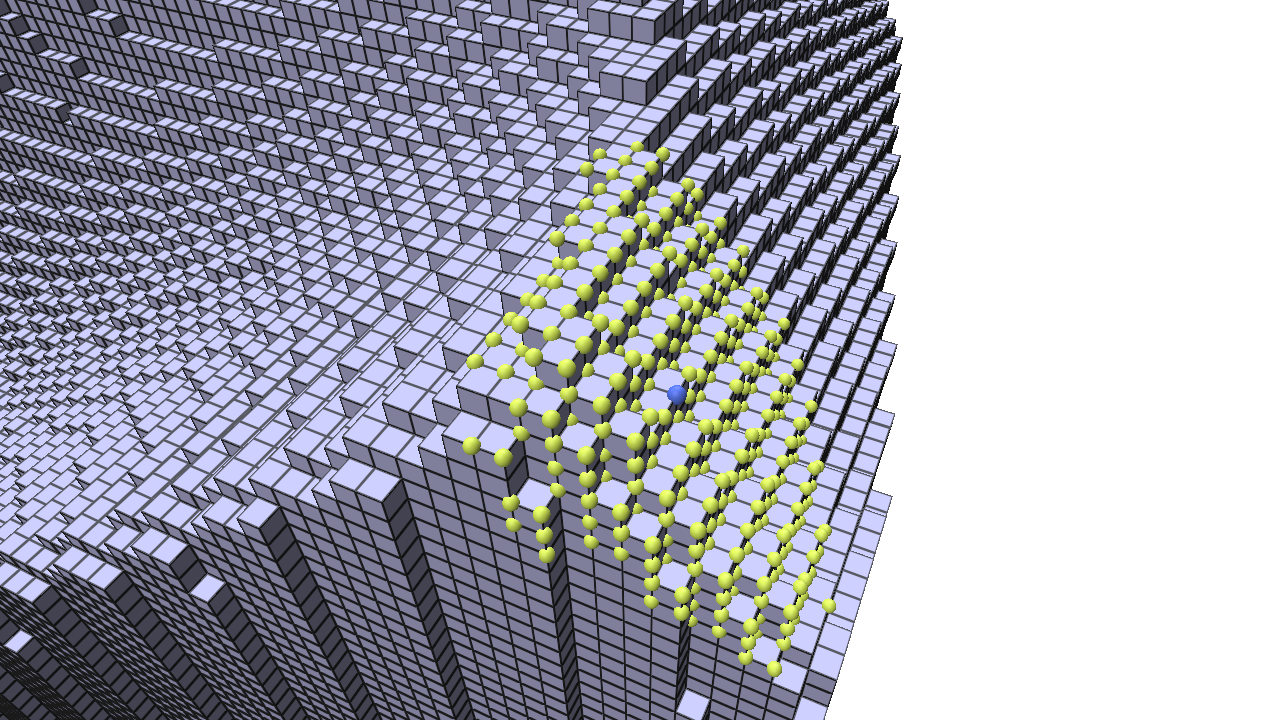
\includegraphics[width=0.4\textwidth]{pictures/visibility_from_given_point_r_10} &
            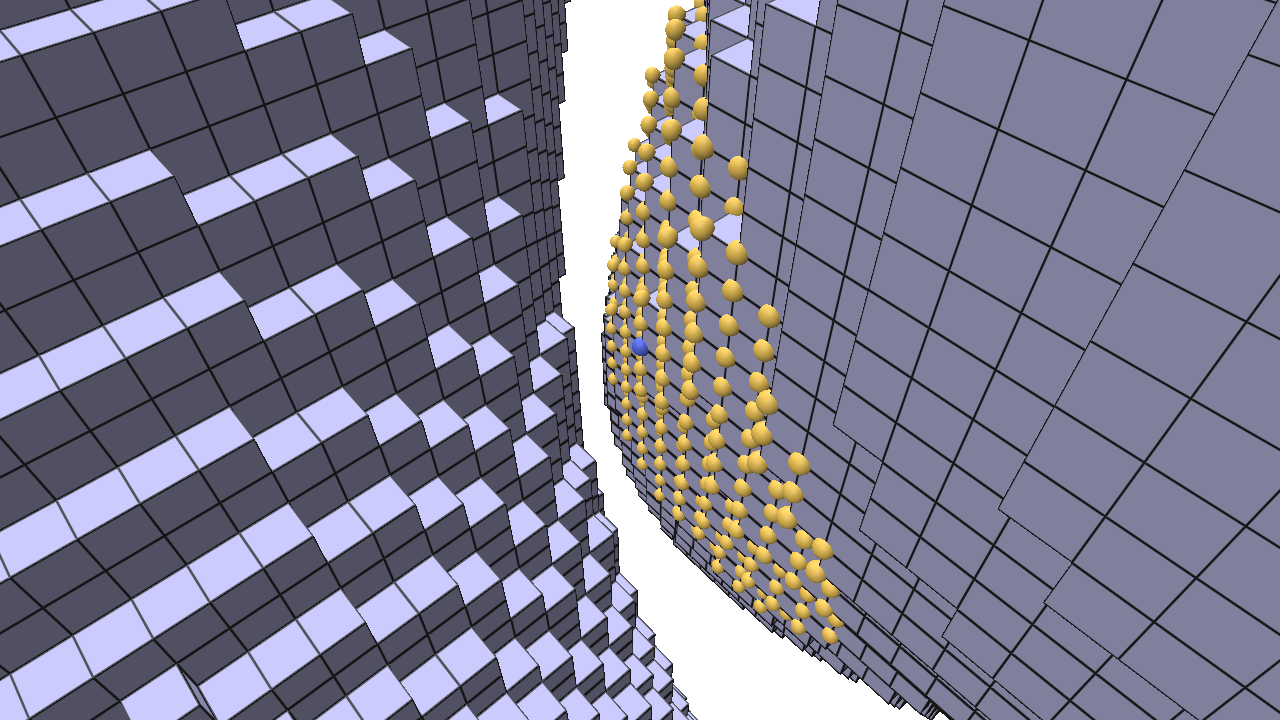
\includegraphics[width=0.4\textwidth]{pictures/visibility_aware_of_features}
        \end{tabular}
        \caption{Examples of visibility on a fandisk and a torus knot. First one is on the edge
        of a fandisk, where the visibility stops at the edges. The other one is in the interior
        of a torus knot, where we can see that the visibility is feature-aware and doesn't see
        the other side of the torus' branch.}
        \label{fig:visibility-results}
    \end{figure}
%
%    \begin{figure}
%        \begin{center}
%            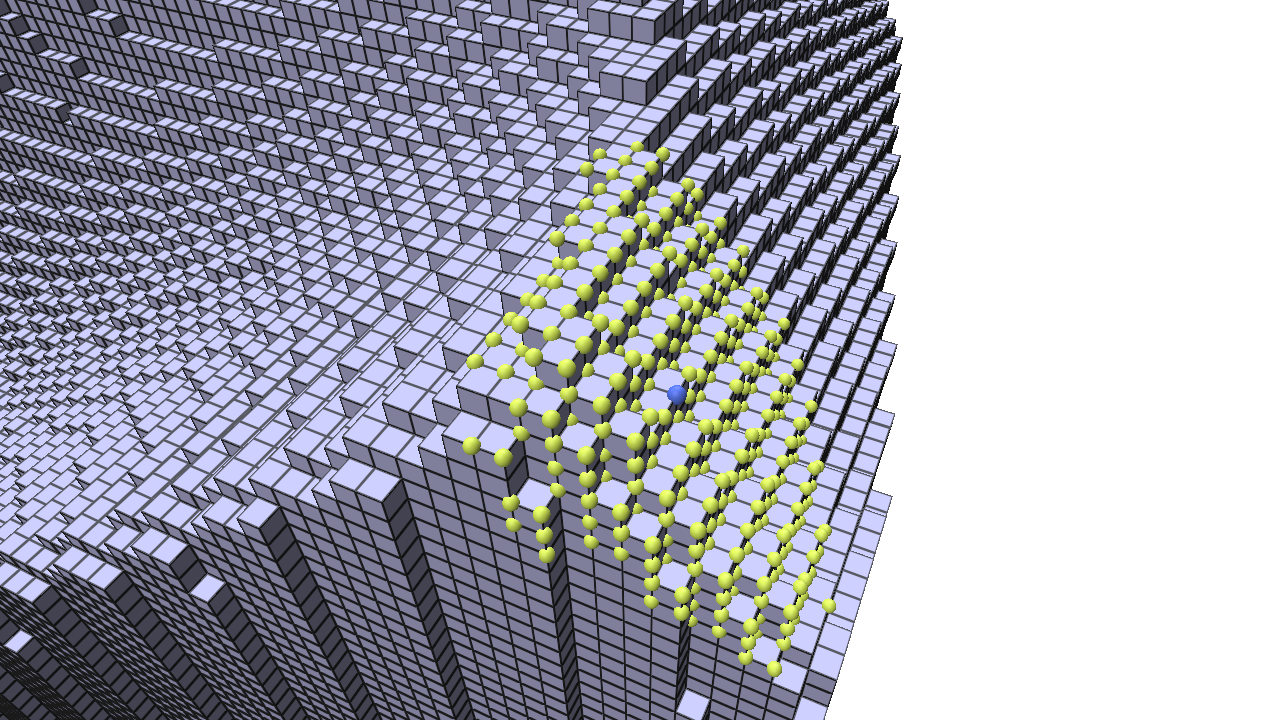
\includegraphics[width=0.8\textwidth]{pictures/visibility_from_given_point_r_10}
%            \caption{Visibility of a point on an edge of a fandisk}
%            \label{fig:visibility-fandisk}
%        \end{center}
%    \end{figure}
%    \begin{figure}
%        \begin{center}
%            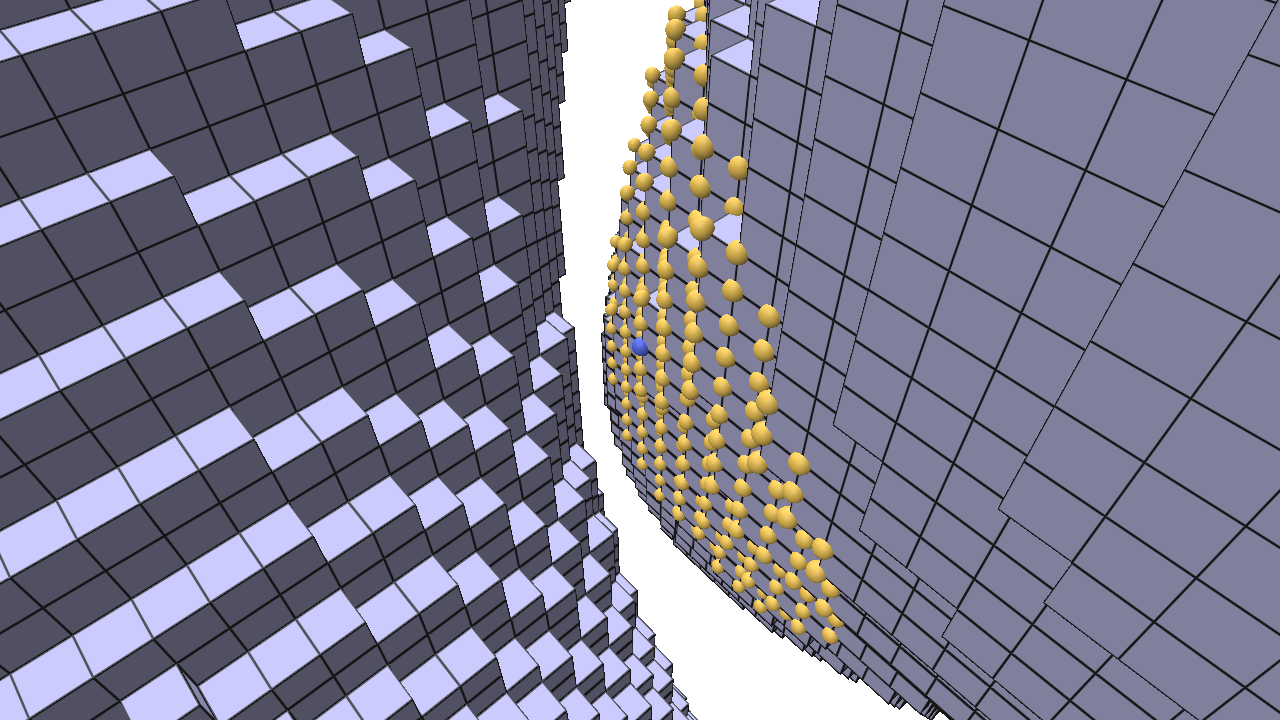
\includegraphics[width=0.8\textwidth]{pictures/visibility_aware_of_features}
%            \caption{Visibility of a point on a torus knot (the visibility is feature-aware)}
%            \label{fig:visibility-torus-knot}
%        \end{center}
%    \end{figure}


    % Quantitative results

    \begin{figure}
        \begin{tikzpicture}
            \centering
            \begin{axis}[
                width=0.8\textwidth,
                legend columns=3,
                xlabel={Gridstep},
                ylabel={Mean distance},
                x dir=reverse,
                legend pos=north west,
                ymajorgrids=true,
                grid style=dashed,
                ymax=70,
                ymode=log,
                xmode=log,
                log ticks with fixed point,
            ]

                \addplot[
                    color=cyan,
                ] coordinates {
                    (0.0625,7.61948)(0.125,5.49755)(0.25,3.97418)(0.375,3.00921)(0.5,2.85702)(0.625,2.34448)(0.75,1.85023)(0.875,2.16868)(1.0,1.85023)
                };
                \addlegendentry{sphere1}
                \addplot[
                    color=red,
                ] coordinates {
                    (0.0625,38.1045)(0.125,26.8765)(0.25,19.6747)(0.375,16.6192)(0.5,14.0867)(0.625,12.5062)(0.75,11.3734)(0.875,10.2845)(1,8.90781)
                };
                \addlegendentry{goursat}
                \addplot[
                    color=violet,
                ] coordinates {
                    (0.0625,25.5024)(0.125,18.2364)(0.25,12.3975)(0.375,9.41303)(0.5,8.69558)(0.625,7.37667)(0.75,6.82131)(0.875,6.05735)(1,6.33877)
                };
                \addlegendentry{torus}
                \addplot[
                    color=MyGreen,
                ] coordinates {
                    (0.0625,27.9287)(0.125,17.5104)(0.25,10.8007)(0.375,8.69514)(0.5,7.26074)(0.625,6.2309)(0.75,5.6897)(0.875,5.28197)(1,4.96098)
                };
                \addlegendentry{leopold}
                \addplot[
                    color=yellow!80!black,
                ] coordinates {
                    (0.0625,41.9816)(0.125,27.7104)(0.25,18.2339)(0.375,14.6475)(0.5,12.3618)(0.625,9.55647)(0.75,9.83208)(0.875,7.51861)(1,7.99732)
                };
                \addlegendentry{rcube}
                \addplot [
                    color=black,
                    thick,
                    domain=0.0625:1,
                    samples=100,
                ] {x^(-0.5)};
                \addlegendentry{$\sqrt{h}=\sqrt{\frac{1}{x}}$}
            \end{axis}
        \end{tikzpicture}
        \caption{Mean Visibility Distance as a Function of Grid Resolution}
        \label{fig:meanvisibility-gridstep}
    \end{figure}

    \begin{figure}[t]
        \begin{tikzpicture}
    \centering
    \begin{axis}[
        width=0.8\textwidth,
        height=0.55\textwidth,
        %xlabel={\#Pointels},
        ylabel={Computation Time (ms)},
        legend pos=north west,
        ymajorgrids=true,
        grid style=dashed,
        ymode=log,
        xmode=log,
        log ticks with fixed point,
    ]

        \addlegendimage{
            black,
            only marks,
            mark=square,
            mark options={solid}
        }
        \addlegendentry{Breadth First}
        \addlegendimage{
            black,
            only marks,
            mark=halfcircle,
            mark options={solid}
        }
        \addlegendentry{Our version}

        \addlegendimage{only marks, mark=*, color=red, mark size=3pt}
        \addlegendentry{Radius 10}
        \addlegendimage{only marks, mark=*, color=MyGreen, mark size=3pt}
        \addlegendentry{Radius 20}
        \addlegendimage{only marks, mark=*, color=blue, mark size=3pt}
        \addlegendentry{Radius 30}

        \addlegendimage{color=black,thick};
        \addlegendentry{$0.01\times x\sqrt{x}$}

        \addplot+[
            red,
            only marks,
            mark=halfcircle,
            mark options={solid}
        ] table[row sep=crcr] {
            % torus
            10624 2246.69\\
            4968 793.426\\
            2584 328.535\\
            1840 190.401\\
            1176 93.2502\\
            912 78.7981\\
            624 56.3769\\
            % rcube
            28568 10193.5\\
            12632 4004.92\\
            7088 2010.63\\
            4664 1188.73\\
            3080 755.754\\
            2408 545.347\\
            1736 366.541\\
            % sphere9
            24320 11169.1\\
            10760 4720.44\\
            6056 2397.79\\
            3944 1380.38\\
            2648 874.979\\
            2000 580.0\\
            1520 415.373\\
            % leopold
            8336 3196.55\\
            3720 1268.46\\
            2104 639.305\\
            1336 342.873\\
            928 177.54\\
            680 112.142\\
            520 87.0747\\
            % goursat
            37592 12335.6\\
            16712 5582.38\\
            9512 2976.21\\
            6056 1731.32\\
            4088 990.78\\
            3032 788.507\\
            2456 548.66\\
            % d20
            97844 49226.3\\
            390235 181322\\
        };
        \addplot+[
            MyGreen,
            only marks,
            mark=halfcircle,
            mark options={solid}
        ] table[row sep=crcr] {
            % torus
            10624 9522.43\\
            4968 2876.81\\
            2584 1152.25\\
            1840 635.332\\
            1176 347.973\\
            912 304.801\\
            624 250.126\\
            % rcube
            28568 70137.9\\
            12632 26063.0\\
            7088 11985.8\\
            4664 6239.51\\
            3080 3468.31\\
            2408 2059.84\\
            1736 1254.2\\
            % sphere9
            24320 86616.9\\
            10760 26605.7\\
            6056 11813.5\\
            3944 6516.92\\
            2648 3564.03\\
            2000 1949.32\\
            1520 1244.89\\
            % leopold
            8336 18125.5\\
            3720 5157.11\\
            2104 2029.09\\
            1336 896.186\\
            928 446.136\\
            680 306.651\\
            520 259.078\\
            % goursat
            37592 76316.3\\
            16712 27747.3\\
            9512 13608.6\\
            6056 7140.03\\
            4088 3704.52\\
            3032 2624.2\\
            2456 1422.6\\
            % d20
            97844 378906\\
            390235 1747780\\
        };
        \addplot+[
            blue,
            only marks,
            mark=halfcircle,
            mark options={solid}
        ] table[row sep=crcr] {
            % torus
            10624 18283.5\\
            4968 4957.93\\
            2584 2133.36\\
            1840 1292.53\\
            1176 922.51\\
            912 863.731\\
            624 813.638\\
            % rcube
            28568 188784.0\\
            12632 62237.1\\
            7088 24874.9\\
            4664 9043.39\\
            3080 4407.09\\
            2408 2641.04\\
            1736 1820.31\\
            % sphere9
            24320 227432.0\\
            10760 69706.8\\
            6056 25408.9\\
            3944 10094.7\\
            2648 5269.56\\
            2000 2948.16\\
            1520 2082.02\\
            % leopold
            8336 45045.4\\
            3720 8638.42\\
            2104 3238.48\\
            1336 1731.9\\
            928 1122.69\\
            680 928.084\\
            520 890.592\\
            % goursat
            37592 257981.0\\
            16712 84729.7\\
            9512 36298.8\\
            6056 15640.2\\
            4088 6662.17\\
            3032 4431.71\\
            2456 2621.98\\
            % d20
            97844 1157400\\
            390235 5493200\\
        };
        \addplot+[
            red,
            only marks,
            mark=square,
            mark options={solid}
        ] table[row sep=crcr] {
            % torus
            10624 6658.15\\
            4968 2740.74\\
            2584 1198.02\\
            1840 853.906\\
            1176 456.784\\
            912 373.028\\
            624 229.479\\
            % rcube
            28568 17837.4\\
            12632 7512.6\\
            7088 4005.5\\
            4664 2522.87\\
            3080 1458.22\\
            2408 1164.01\\
            1736 770.449\\
            % sphere9
            24320 17922.8\\
            10760 7845.85\\
            6056 4431.68\\
            3944 2840.96\\
            2648 1774.39\\
            2000 1292.66\\
            1520 867.89\\
            % leopold
            8336 6268.17\\
            3720 2697.19\\
            2104 1489.4\\
            1336 871.987\\
            928 588.548\\
            680 363.434\\
            520 237.277\\
            % goursat
            37592 23416.9\\
            16712 9923.63\\
            9512 5446.57\\
            6056 3256.35\\
            4088 2008.14\\
            3032 1467.76\\
            2456 1107.06\\
            % d20
            97844 73606.0\\
            390235 337851.0\\
        };
        \addplot+[
            MyGreen,
            only marks,
            mark=square,
            mark options={solid}
        ] table[row sep=crcr] {
            % torus
            10624 18932.3\\
            4968 6555.12\\
            2584 2621.4\\
            1840 1571.18\\
            1176 759.752\\
            912 510.296\\
            624 323.584\\
            % rcube
            28568 81041.4\\
            12632 30169.2\\
            7088 14369.6\\
            4664 7318.29\\
            3080 4377.33\\
            2408 2255.89\\
            1736 1743.95\\
            % sphere9
            24320 108696.0\\
            10760 29433.6\\
            6056 11092.9\\
            3944 5535.89\\
            2648 2759.14\\
            2000 1770.88\\
            1520 1103.44\\
            % leopold
            8336 24782.2\\
            3720 7521.02\\
            2104 2976.49\\
            1336 1296.38\\
            928 777.747\\
            680 455.317\\
            520 283.182\\
            % goursat
            37592 124066.0\\
            16712 45347.2\\
            9512 22445.1\\
            6056 12308.8\\
            4088 7370.63\\
            3032 5317.86\\
            2456 3356.28\\
            % d20
            97844 368339.0\\
            390235 1784570.0\\
            };
        \addplot+[
            blue,
            only marks,
            mark=square,
            mark options={solid}
        ] table[row sep=crcr] {
            % torus
            10624 32025.4\\
            4968 9426.13\\
            2584 3596.87\\
            1840 1975.03\\
            1176 930.202\\
            912 626.321\\
            624 402.24\\
            % rcube
            28568 183072.0\\
            12632 57696.6\\
            7088 22998.7\\
            4664 8654.47\\
            3080 5090.0\\
            2408 2538.87\\
            1736 2004.77\\
            % sphere9
            24320 124004.0\\
            10760 31699.4\\
            6056 11704.3\\
            3944 6068.31\\
            2648 2885.91\\
            2000 1888.12\\
            1520 1170.45\\
            % leopold
            8336 31540.8\\
            3720 8280.03\\
            2104 3236.58\\
            1336 1451.9\\
            928 807.249\\
            680 477.556\\
            520 299.46\\
            % goursat
            37592 245584.0\\
            16712 82093.2\\
            9512 37091.0\\
            6056 18530.7\\
            4088 9711.66\\
            3032 6214.95\\
            2456 3523.63\\
            % d20
            97844 778491.0\\
            390235 4409340.0\\
            };
        \addplot[
            color=black,
            thick,
            domain=500:300000,
            samples=200,
        ] {0.01*x^(1.5)};
    \end{axis}
\end{tikzpicture}

        \caption{Computation Time of Visibility as a Function of pointels amount. We compare the computation time of
        the naive breadth first visibility algorithm against our version using intervals. We input the same radius to
        both versions (10, 20, 30) and test it on 6 different figures (goursat, torus, rcube, sphere9, leopold, d20)
        with various gridsteps, giving us figures with pointel amounts ranging from 520 to 390235.}
        \label{fig:meanvisibility-computationComplexity}
    \end{figure}
